\documentclass[11pt]{article}

\usepackage[utf8]{inputenc}
\usepackage[T1]{fontenc}
\usepackage[a4paper,margin=2.5cm]{geometry}
\usepackage{amsmath,amssymb,amsthm,mathtools,bm,dsfont}
\usepackage{booktabs,array,tabularx,multirow}
\usepackage{graphicx,subcaption,float}
\usepackage[dvipsnames]{xcolor}
\usepackage{microtype}
\usepackage{enumitem}
\usepackage[hidelinks]{hyperref}
\usepackage[nameinlink]{cleveref}

% ---- notation of the Dipole-lets paper (Contreras-Z\'u\~niga et al.) ----
\newcommand{\R}{\mathbb{R}}
\newcommand{\C}{\mathbb{C}}
\newcommand{\F}{\mathcal{F}}
\newcommand{\bk}{\bm{k}}
\newcommand{\bx}{\bm{x}}
\newcommand{\bxi}{\bm{\xi}}
\newcommand{\md}{\mathfrak{D}}
\newcommand{\ind}{\mathds{1}}
\newcommand{\norm}[1]{\lVert #1\rVert}
\newcommand{\abs}[1]{\lvert #1\rvert}
\newcommand{\Real}{\operatorname{Re}}
\newcommand{\code}[1]{\texttt{#1}}
\DeclareMathOperator{\argmin}{arg\,min}
\DeclareMathOperator{\clip}{clip}
\DeclareMathOperator{\sigm}{sigm}

\newtheorem{remark}{Remark}

\title{\textbf{Where the non-dipolar phase lives in the Dipole-let domain, and what a cleaner can do about it}\\[2pt]
\large Results of the MCNO-QSM study\\[2pt]
\normalsize Technical report --- October 2026}
\author{}
\date{}

\begin{document}
\maketitle

\begin{abstract}
\noindent
We study the removal of the non-dipolar part $\psi_N$ and the noise $\varepsilon$ from a single-orientation local-field map $\psi=\psi_D+\psi_N+\varepsilon$ \emph{before} susceptibility inversion, so that the streaking they cause in the eNDI reconstruction is reduced.
Everything is expressed in the Dipole-let domain: $S=JM+1$ coefficients $\md_{j,m}\psi$ built from radial scales $R_j$ and angular windows $A_m$ around the magic cone $\Sigma$.
We report (i) the geometry of $\psi_N$ in that domain: noise is separable by scale (radial), the measured and modelled in-vivo residuals by angle ($\abs D$), so one set of filter gains cannot serve both; (ii) that a field-domain Fourier network trained on noise sits at a measured information floor, and that none of six loss, architecture or data variants moves it; (iii) a zero-training \emph{regime-gated passive Dipole-let filter} placed in front of that network, which lowers the eNDI error on the measured tissue residual from $71.7\%$ to $58.6\%$ (dirty $93.6\%$) without changing the noise-like cases; (iv) four negative results on the remaining failure, strong compact sources such as a calcification (amplitude gating, a passivity constraint, a source suppressor, plug-and-play refinement inside eNDI); and (v) a data-driven redesign of the decomposition, which improves the phase error but not the eNDI error.
All numbers come from one seed, one training head (RC1) and one simulated test volume (Sim2); no in-vivo data were tested. Limits are stated next to each result and in \cref{sec:limits}.
\end{abstract}

\tableofcontents
\newpage

% =====================================================================
\section{Model, notation and aim}\label{sec:model}

\paragraph{Model.} Following \cite{dipolelets}, the measured local field (in ppm) is
\begin{equation}\label{eq:model}
\psi=\psi_D+\psi_N+\varepsilon,\qquad \psi_D=\Real\,\F^{-1}\big(D\cdot\F\chi\big),\qquad D(\bk)=\tfrac13-\frac{k_z^2}{\norm{\bk}_2^2},
\end{equation}
with the magic cone $\Sigma=\{D=0\}$. $\psi_N$ is the non-dipolar phase (microstructure, anisotropy, remnants) and $\varepsilon$ the noise; $m$ is the brain mask and $w$ the eNDI weight (magnitude). The inversion is the authors' eNDI (\code{ndiCG}); the cleaner only acts on $\psi$.
\emph{Aim:} find an operator $f$ with $f(\psi,m,w)\approx m\odot\psi_D$ such that the eNDI map of $f(\psi)$ is closer to $\chi$ than the eNDI map of $m\odot\psi$.

\paragraph{Dipole-lets.} Radial filters $R_j$ ($j=0,\dots,J-1$) and a low-pass residual $R_{\mathrm{res}}$, with $\sum_jR_j+R_{\mathrm{res}}=1$, and angular windows $A_m$ ($m=0,\dots,M-1$), $\sum_mA_m=1$, defined by thresholds $\delta_0<\dots<\delta_{M-2}$ on $\abs{D}$:
\begin{equation}
\md_{j,m}\psi=\F^{-1}R_jA_m\F\psi,\qquad \md_{\mathrm{res}}\psi=\F^{-1}R_{\mathrm{res}}\F\psi,\qquad \psi=\sum_{j,m}\md_{j,m}\psi+\md_{\mathrm{res}}\psi,
\end{equation}
$S=JM+1$ segments, indexed by $s$. All results use $J=3$, $M=3$, $\delta=0.05$, $\delta_1=1/3$, error-function windows, starlet scale $\sigma=0.5$ voxel (so $A_0$ is the near-cone band $\abs D<0.05$, $A_1$ the band $0.05<\abs D<1/3$, $A_2$ the rest). We also use the \emph{split residual} $\md_{\mathrm{res},m}\psi=\F^{-1}R_{\mathrm{res}}A_m\F\psi$, which replaces $\md_{\mathrm{res}}$ by $M$ pieces and gives $S'=JM+M=12$ segments.
A \emph{passive Dipole-let filter} with gains $g\in[0,1]^S$ is
\begin{equation}\label{eq:passive}
\mathcal P_g\psi=m\odot\sum_{s}g_s\,\md_s\psi,
\end{equation}
which can only attenuate segments (no gain above one, none negative).

\paragraph{Two regimes.} We distinguish \emph{noise-like} $\psi_N+\varepsilon$ (white, rough, as in the simulated Sim2) and \emph{real-like} $\psi_N$ (tissue residual, STI and off-diagonal terms measured or modelled on RC1).

% =====================================================================
\section{Data and evaluation protocol}\label{sec:protocol}

\paragraph{Data.} RC1 is the FANSI challenge-1 head ($160^3$, $1.06$\,mm, TE\,25\,ms, $B_0$\,2.89\,T) with the COSMOS susceptibility, the measured tissue phase \code{phs\_tissue} and the STI tensor. Sim2 is a $164\times205\times205$ simulation at 7\,T (TE\,8\,ms) with a calcification (37 voxels below $-0.5$\,ppm, $\chi$ down to $-2.03$\,ppm) and a measured-like $\psi_N+\varepsilon$ (rms $0.0037$\,ppm, $84.7\%$ of its energy above $0.2$ cycles/mm). Sim2 is \emph{only a test volume}: it is never used for training, selection or design choices; thresholds and gains are read from RC1.
The clean target is always $y=m\odot\psi_D(\chi)$ with the correctly aligned kernel (the FANSI kernel is misaligned for odd matrix sizes).

\paragraph{Experiments (RC1, from the Dipole-lets notebook).}
\Cref{tab:exps} lists the fields on which methods are compared. exp7 is the only \emph{measured} non-dipolar phase; exp8 and exp9 are modelled, and the filters of \cref{sec:regime} are fitted on noisy versions of exactly those two kinds of residual, so exp8 and exp9 are in-sample for the fit while exp7 is held out (same head, different residual).
\begin{table}[h]\centering\small
\begin{tabular}{@{}lp{12.2cm}@{}}
\toprule
exp1 & $\psi=\psi_D(\chi_{\mathrm{COSMOS}})$ masked (noiseless: any change is damage)\\
exp3 & $\psi_D$ with complex noise at SNR\,40 \\
exp5, exp6 & $\psi_D$ plus cylinders (r\,=\,8, $\pm0.5$\,ppm) / spheres (r\,=\,4, $\pm0.33$\,ppm) added to the phase: \emph{strong localized sources} \\
exp7 & measured \code{phs\_tissue} (the real residual $\psi=\psi_D+\psi_N$) \\
exp8, exp9 & the STI field $p_{33}-(p_{13}+p_{23})$ / the clean field minus the off-diagonal term, $\psi_D-p_Q$ \\
Sim2 real & \code{Frequency.nii}: the measured-like $\psi_N+\varepsilon$, calcification included \\
Sim2 forward & $\psi_D(\chi_{\mathrm{Sim2}})$ plus noise (SNR\,100, calibrated, 40), plus phase jumps, plus $\chi$ spheres \\
\bottomrule
\end{tabular}
\caption{Experiments.}\label{tab:exps}
\end{table}

\paragraph{Score.} eNDI (\code{ndiCG}, $\alpha=10^{-5}$, zero-padded to $192^3$ for RC1 and $256^3$ for Sim2), run for a \emph{fixed} number of iterations, \textbf{25} (history index 25 of the NRMSE curve, i.e.\ 26 gradient steps), \emph{not} with the automatic stop. The score is $\mathrm{NRMSE}=100\,\norm{m\odot(\hat\chi-\chi)}/\norm{m\odot\chi}$. Fixed iterations are used because the dirty fields diverge after $4$--$17$ iterations and the stop fires at very different iterations for different fields, which confounds comparisons. Phase NRMSE ($\norm{m\odot(\hat\psi-\psi_D)}/\norm{m\odot\psi_D}$) is reported where useful but is not the criterion (\cref{sec:floor}). Oracle (eNDI of $y$): $35.8\%$ (RC1), $43.1\%$ (Sim2).

\paragraph{Rules followed.} Success criteria were written down before each run (they are quoted below); a negative result is recorded as negative; every number is a single seed and a single volume unless a spread is given.

% =====================================================================
\section{Geometry of the non-dipolar phase in the Dipole-let domain}\label{sec:geometry}

\subsection{Angular versus radial separability}
For each regime we accumulate, on a grid of $24$ radial bins ($\norm\bk$ in cycles/voxel) $\times\,12$ bins of $\abs D$, the cell energies $E_b=\sum\abs{\hat y}^2$, $E_{bd}=\sum\Real(\hat y\,\overline{\hat\psi})$, $E_d=\sum\abs{\hat\psi}^2$ ($\hat y,\hat\psi$ the transforms of the clean and the dirty masked field). The best passive scalar gain of a cell is $g=\clip(E_{bd}/E_d,0,1)$.
\Cref{fig:gains} shows $g$ for the three regimes.
\begin{figure}[t]\centering
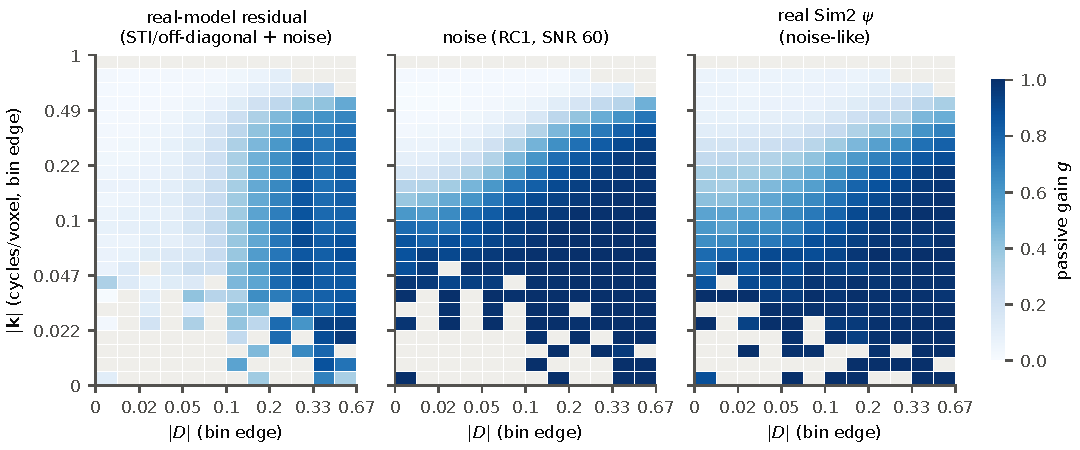
\includegraphics[width=\linewidth]{figures/fig_gain_maps.pdf}
\caption{Best passive gain per cell of the $(\norm\bk,\abs D)$ plane (light grey: cell without energy). Left: modelled in-vivo residuals (STI and off-diagonal terms plus noise, RC1): the gain depends on $\abs D$ and hardly on $\norm\bk$. Middle: white noise on RC1: the gain depends on $\norm\bk$ (about 1 below $0.1$ cycles/voxel, falling to $\lesssim0.1$ above $0.4$ for $\abs D<0.1$) and weakly on $\abs D$. Right: the noise-like $\psi$ of the real Sim2.}\label{fig:gains}
\end{figure}
The two regimes are separated by different variables:
\begin{itemize}[leftmargin=1.5em,itemsep=1pt]
\item \textbf{Real-like $\psi_N$ is angular.} The share of the energy that lies close to $\Sigma$ is far higher than for the clean field (\cref{tab:cone}); the local signal-to-residual ratio $\abs{\hat y}^2/\abs{\hat\psi_N}^2$ is $-13$ to $-17$\,dB in $\abs D<0.05$ at \emph{every} $\norm\bk$ (even below $0.03$ cycles/mm), about $-9$\,dB in $0.05<\abs D<0.1$, and $+4$ to $+11$\,dB above $0.2$. The optimal gain rises from $\approx0.1$ at $\abs D<0.05$ through $0.4$ at $0.15$ and $0.7$ at $0.27$ to $0.85$ at $0.33$, independent of scale. This is the premise of the Dipole-lets paper (non-dipolar content in the near-cone bands at every scale).
\item \textbf{Noise is radial.} For Sim2's noise-like $\psi$ the local signal-to-residual ratio changes with $\norm\bk$ ($+25$\,dB below $0.03$, $0$\,dB at $0.2$--$0.3$, $-12$\,dB above $0.4$ cycles/mm) and only $10$--$15$\,dB along $\abs D$; the three radial scales of the decomposition resolve only $\norm\bk\gtrsim0.1$ cycles/voxel and the residual carries $78.6\%$ of the true-field energy.
\end{itemize}
\begin{table}[h]\centering\small
\begin{tabular}{@{}lrr@{}}
\toprule
 & $\abs D<0.05$ & $\abs D<0.1$ \\
\midrule
clean field $y$ (RC1) & 0.21 & 0.88 \\
noise $\varepsilon$ & 12 & 24 \\
real tissue residual & 13 & 26 \\
STI term & 20 & 37 \\
off-diagonal term & 11 & 21 \\
\bottomrule
\end{tabular}
\caption{Share (\%) of the energy that lies in the near-cone region, RC1.}\label{tab:cone}
\end{table}
\begin{remark}
The cone share alone does not discriminate noise from real residuals (white noise puts $12\%$ in $\abs D<0.05$, the real residual $13\%$); what does is the \emph{scale dependence}: the local excess of cone energy over its white-noise expectation falls by a factor $\sim10$ from the finest to the coarsest scale for noise and is flat across scales for the real residuals (\cref{sec:regime}).
\end{remark}

\subsection{An information floor in the field domain}\label{sec:floor}
Within each cell the best \emph{scalar} filter fitted on the volume itself (an optimistic oracle) leaves $27.27\%$ phase error on Sim2; the trained network leaves $27.16\%$, and a best-fit linear filter with one gain per segment leaves $26.44\%$ against the network's $26.26\%$. The network is at, and in the near-cone cells below, that floor: for noise-like $\psi_N+\varepsilon$ nothing is left to extract with a linear-in-cell or per-segment filter, and a weighted-L2 loss of any kind has the same minimiser (the conditional mean).
Two consequences matter below. (a) Re-weighting the loss cannot help (confirmed, \cref{sec:network}). (b) \textbf{Phase NRMSE does not predict eNDI error}: the tissue-only network reduces the phase error on Sim2 ($42.2\to37.4\%$) yet its eNDI error is $60.6\%$ against $52.6\%$ for the dirty field; four different decompositions in \cref{sec:design} differ by $3$ points of phase error and $<0.9$ points of eNDI error. All claims are therefore made in eNDI.

% =====================================================================
\section{The field-domain network (stage B) and its plateau}\label{sec:network}

Stage B is the Dipole-let Fourier network of the companion report: a residual FNO whose spectral weights are tied to the $S=10$ Dipole-let segments (complex channel mixing per segment, modulated by a small network of $D(\bk)$, $\norm\bk$, $\hat\bk$), 67{,}305 parameters, $\hat\psi_D=m\odot(\psi-\widehat{\psi}_N)$. The recipe that works on Sim2 is \emph{noise}: RC1 patches of $96^3$ with complex noise at SNR\,40--200 (plus $20\%$ identity examples, \emph{noise\_clean}, so that clean fields are left alone), trained on one head. We call this network $B$.
\begin{table}[h]\centering\small
\begin{tabular}{@{}lrr@{}}
\toprule
 & auto-stop eNDI & 25 fixed it. \\
\midrule
dirty (masked) & 52.60 & 53.94 \\
low-pass $\sigma=0.5$ (tuned on the target) & 49.03 & -- \\
all nine artifact families (mix, 3 seeds) & $49.05\pm0.19$ & 50.0 \\
\textbf{noise} (3 seeds) & $\mathbf{46.96\pm0.04}$ & 47.28 \\
noise + band-normalized spectral loss & 47.47 & -- \\
noise + local dilated conv in each block (3 seeds) & $46.43\pm0.45$ & -- \\
noise + U-Net branch (3 seeds; branch inert) & $46.67\pm0.22$ & -- \\
noise\_clean (identity examples) & -- & \textbf{47.31} \\
noise\_clean + 85 AHEAD anatomies & -- & 47.71 \\
noise\_clean + Dipole-let sensitivity-weighted loss & -- & 47.27 \\
noise\_clean + calcification-shell family & -- & 47.36 \\
oracle & 44.22 & 43.10 \\
\bottomrule
\end{tabular}
\caption{eNDI NRMSE (\%) on the real Sim2 (single volume). The first column is the early series with the automatic stop (masked), the second the fixed-iteration protocol used from here on. Every variant of the noise recipe lies within $\sim0.5$ points of it.}\label{tab:plateau}
\end{table}
\Cref{tab:plateau} summarizes a long series: neither a loss that re-weights bands or Dipole-let segments (with measured eNDI sensitivities $g_s$), nor a local convolution, a U-Net branch, 85 additional anatomies, or a training family modelled on the calcification changes the result beyond $0.5$ points. Capacity is not the limit: the same network removes phase-additive localized artifacts of its own making to $97\%$ on fresh draws, and the train and held-out noise ratios are equal ($0.466$ and $0.449$, no overfitting). Mixing structured families into the recipe is \emph{worse} on Sim2 ($49.05$), a negative task interference. The calcification family, the one designed for Sim2's failure, does not recover the field in the $3$\,mm shell around the source (relative error $1.02$, gain $0.27$), because the \emph{input} there keeps only $32\%$ of the true field.

% =====================================================================
\section{A regime-gated passive Dipole-let filter in front of the network}\label{sec:regime}

\subsection{Linear Dipole-let filters on real-like residuals}
With no training, one real gain per segment fitted by least squares on RC1's modelled residuals (STI and off-diagonal terms with noise at SNR\,100, \emph{never} the measured tissue) and applied to the measured tissue residual exp7 already removes most of the damage (\cref{tab:linear}). Splitting the residual by angle, $\md_{\mathrm{res}}\to\md_{\mathrm{res},m}$, is worth $1.4$--$2.7$ eNDI points on exp7--9 (the phase gain was $2.5$--$4$ points); in the phase proxy more radial scales ($J=4,5$) give the same linear gain as the split and saturate at $J=6$, and in eNDI the $15$- and $16$-segment filters are within $0.3$ of the $12$-segment one; none of these changes the result on noise-like fields.
\begin{table}[h]\centering\small
\begin{tabular}{@{}lccc@{}}
\toprule
filter (gains from the other two real types) & exp7 & exp8 & exp9 \\
\midrule
dirty & 93.6 & 67.7 & 83.3 \\
network $B$ (noise\_clean) & 71.4 & 60.9 & 75.9 \\
cone notch $\abs D<0.15$ on the dirty field & 64.8 & 52.8 & 60.7 \\
10 segments ($J=3,M=3$) & 62.2 & 55.6 & 59.5 \\
\textbf{12 segments (split residual)} & \textbf{59.7} & \textbf{54.2} & \textbf{56.8} \\
15 segments ($J=4$ + split) & 59.6 & 54.2 & 56.7 \\
16 segments ($J=5,M=3$) & 59.8 & 54.4 & 57.1 \\
\bottomrule
\end{tabular}
\caption{Zero-training linear Dipole-let filters, eNDI NRMSE (\%) at 25 iterations. Fitted gains of one real type are applied to the others (exp7 is never fitted).}\label{tab:linear}
\end{table}
A 12-parameter linear filter beats the trained network $B$ on the real residuals by $12$, $7$ and $19$ points, and the trained network behaves on them like a radial Wiener filter. The price: the gains of the \emph{real} regime applied to Sim2's noise-like $\psi$ give $57$--$58\%$ (worse than dirty, $53.9$), while the gains fitted on noise give $49.2$ and $69$--$71$ on exp7/exp9: choosing the wrong regime costs $8$--$12$ points either way.

\subsection{The regime map and the gated filter}\label{sec:gate}
The regime must be read from the input. Let $G_\rho$ be a Gaussian of $\rho=6$ voxels and, for the detail scale $j$,
\begin{equation}\label{eq:excess}
\phi_j(\bx)=\log\frac{G_\rho\!*\!(\md_{j,0}\psi)^2}{G_\rho\!*\!\sum_{m\ge1}(\md_{j,m}\psi)^2}-\log\mu_j,\qquad \mu_j=\frac{\norm{R_jA_0}^2}{\sum_{m\ge1}\norm{R_jA_m}^2},
\end{equation}
the local log excess of near-cone energy over its white-noise expectation ($\phi_j=0$ for white noise). Medians of $\exp\phi_j$ over $96^3$ patches: noise $0.15$--$0.78$ at the finest scale falling to $0.06$--$0.09$ at the coarsest; the real Sim2 $\psi$ $0.47/0.26/0.13$; tissue, STI and off-diagonal residuals flat across scales ($0.50/0.43/0.42$, $0.34/0.36/0.38$, $0.24/0.26/0.28$). The coarsest detail scale separates the regimes with a margin of $\sim1.4$. We use it only:
\begin{equation}\label{eq:gate}
r(\bx)=\sigm\!\big(6\,\phi_{2}(\bx)+c\big),\qquad c=-6\ln0.22=9.0848,
\end{equation}
($r=0.5$ at an excess of $0.22$; $r\approx0.00$ on noise, $0.05$ on the mean of the real Sim2, $0.93$/$0.89$/$0.78$ on exp7/exp8/exp9). \textbf{Stage A} removes the real-regime correction where the gate is on:
\begin{gather}\label{eq:stageA}
\mathcal A\psi=m\odot\Big(\psi-r\odot\sum_{s}(1-g_s)\,\md_s\psi\Big),\
g=\argmin_{g\in[0,1]^{S'}}\sum_{f}\Big\lVert m\odot\Big(\sum_sg_s\md_s\psi^{(f)}-\psi_D\Big)\Big\rVert^2,
\end{gather}
with the $12$ segments of the split residual, $f$ running over the two modelled residual types (STI and off-diagonal), $\psi^{(f)}$ their noisy versions on RC1 at SNR\,100 and the bound $g\in[0,1]$ (passive filter, \cref{eq:passive}). The fitted gains are
\begin{equation}
g=(0,\,0,\,0.40,\;0,\,0.74,\,1.0,\;0,\,0.77,\,0.83,\;0,\,0.67,\,0.92)
\end{equation}
for $(\md_{0,0},\md_{0,1},\md_{0,2},\md_{1,0},\dots,\md_{\mathrm{res},2})$: the near-cone band $\abs D<0.05$ is removed at every scale and in the residual, the band $0.05<\abs D<1/3$ is attenuated (removed entirely at the finest scale), the far band is kept. A first fit without the bound has gains in $[-1.4,1.3]$ and costs $\approx1$ point less on exp7--9 but amplifies strong sources (\cref{sec:strong}); the bound costs about one point and halves that damage.
\textbf{The cascade} is $\widehat\psi_D=B(\mathcal A\psi)$: stage A (no training; gains and gate read from RC1 only) followed by the unchanged network $B$. In the noise regime ($r\to0$) it reduces to $B$.

\subsection{Results}
\Cref{tab:main} and \cref{fig:main} compare the dirty field, $B$ alone, the joint network that learns the gains and the gate jointly with the data (12 segments, trained on the mixture of noise and modelled residuals) and the cascade. Criteria fixed beforehand: exp7 $\le63$; no harm on noise-like data (real Sim2 $\le47.8$, forward Sim2 fields within $0.5$ of $B$, exp1 $\le36.8$, exp3 within $1.0$); exp8 and exp9 at least $5$ points better than $B$.
\begin{table}[h]\centering\small
\begin{tabular}{@{}lrrrrr@{}}
\toprule
 & dirty & $B$ & joint net & stage A alone & \textbf{cascade} $B\!\circ\!\mathcal A$ \\
\midrule
exp7 (measured tissue) & 93.60 & 71.69 & \textbf{56.58} & 61.37 & 58.63 \\
exp8 (STI) & 67.69 & 61.15 & \textbf{50.40} & 52.79 & 52.35 \\
exp9 (off-diagonal) & 83.33 & 76.33 & \textbf{53.60} & 62.09 & 60.46 \\
\midrule
Sim2 real & 53.94 & \textbf{47.48} & 48.62 & 54.62 & 48.72 \\
Sim2 fwd SNR\,100 & 61.48 & \textbf{46.69} & 46.97 & 61.11 & 46.86 \\
Sim2 fwd SNR cal. & 67.52 & \textbf{47.44} & 47.90 & 68.35 & 47.71 \\
Sim2 fwd SNR\,40 & 121.45 & \textbf{52.13} & 55.37 & 113.68 & 52.48 \\
Sim2 fwd jumps & 66.81 & \textbf{48.43} & 50.58 & 67.00 & 48.57 \\
Sim2 fwd $\chi$ spheres & 70.57 & \textbf{51.68} & 51.87 & 69.63 & 51.76 \\
exp1 (noiseless) & \textbf{35.76} & 36.11 & 37.54 & 35.77 & 36.11 \\
exp3 (SNR\,40) & 61.15 & \textbf{43.02} & 43.98 & 60.69 & 43.05 \\
\midrule
exp5 (cylinders) & \textbf{94.14} & 116.13 & 169.87 & 105.67 & 113.56 \\
exp6 (phase spheres) & \textbf{35.83} & 46.60 & 68.59 & 65.15 & 62.95 \\
\bottomrule
\end{tabular}
\caption{eNDI NRMSE (\%) at 25 fixed iterations. The cascade equals $B$ within $0.35$ on all forward-simulated fields, exp1 and exp3, lowers the measured residual (exp7) by $13$ points relative to $B$ and exp8/exp9 by $9$/$16$; the joint network is better on exp7--9 but costs $0.2$--$3.2$ points on noise-like data. Real Sim2: $B$ is $47.48$ here and $47.31$ in the trainer's own output (a different outside-the-mask convention).}\label{tab:main}
\end{table}
\begin{figure}[t]\centering
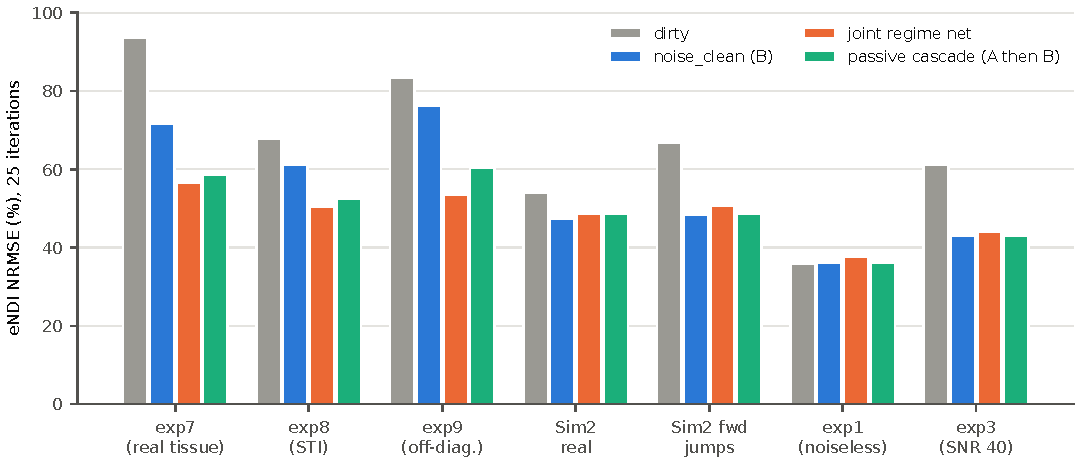
\includegraphics[width=\linewidth]{figures/fig_endi_main.pdf}
\caption{Selected rows of \cref{tab:main} (eNDI NRMSE, lower is better): dirty field, network $B$, joint regime network, passive cascade. The cascade follows $B$ on the noise-like cases and follows the joint network on the real residuals.}\label{fig:main}
\end{figure}
\textbf{Verdict against the criteria.} Met: exp7 ($58.6\le63$); exp8/exp9 ($9$ and $16$ points better than $B$); forward Sim2 fields (largest $+0.35$), exp1 ($36.11$), exp3 ($+0.03$). \emph{Not} met: real Sim2 ($48.72>47.8$, $+1.24$ over $B$). The soft gate and a hard gate ($r>0.5$) agree within $0.9$ everywhere.

% =====================================================================
\section{The remaining failure: strong compact sources}\label{sec:strong}

\paragraph{Localization.} The real-Sim2 loss ($+1.24$ over $B$ for the cascade) comes from the neighbourhood of the calcification: for the unconstrained stage A alone, which was the version localized (the passive one was not re-localized), it sits entirely within $15$\,mm of it. In the field domain that stage A \emph{lowers} the error everywhere ($42.2\to39.6\%$ phase NRMSE; $0.65\times$ inside the gated voxels far from the calcification) and raises it only in the $3$--$8$\,mm ring around it ($1.21\times$). In eNDI (laptop run, history index 24, dirty $53.47$):
applying the unconstrained stage A everywhere $54.91$; only farther than $15$\,mm from the calcification $53.41$ (no harm); only within $15$\,mm $54.95$; only where $r>0.5$ $55.04$. The same happens on the RC1 strong sources exp5/exp6 (stage A alone $198$/$76$ with the unconstrained gains against $94$/$36$ dirty). The filter zeros near-cone content of true fields of compact sources, and the cone-excess gate does not exclude them.

\paragraph{Four remedies, all negative.}
Criteria for stage A alone were fixed before each run (exp5 $\le99$, exp6 $\le40$, exp7 $\le63$, exp8 $\le58$, Sim2 real $\le dirty+0.3$).
\begin{table}[h]\centering\small
\begin{tabular}{@{}lrrrrrr@{}}
\toprule
stage A alone, eNDI@25 (laptop, index 24) & exp5 & exp6 & exp7 & exp8 & exp9 & Sim2 real \\
\midrule
dirty & 93.6 & 36.0 & 92.8 & 67.7 & 83.3 & 53.47 \\
unconstrained gains & 198.1 & 75.6 & 60.2 & 51.9 & 61.1 & 54.91 \\
+ amplitude suppressor, $\sigma=6$ voxels & 157.4 & 51.0 & 60.2 & -- & -- & 54.91 \\
passive gains $g\in[0,1]$ & 104.1 & 63.2 & 61.2 & 52.7 & 61.9 & 54.40 \\
passive + suppressor, $\sigma=2.5$, 0.06--0.10\,ppm & 124.8 & 45.2 & 61.2 & 52.7 & 61.9 & 54.37 \\
\bottomrule
\end{tabular}
\caption{Attempts to protect strong sources. Suppressor: the gate is multiplied by $1-\mathrm{smoothstep}\big((\ell-\ell_0)/(\ell_1-\ell_0)\big)$, $\ell$ the local rms of the field; thresholds read from RC1 only (real residuals and noise stay below $0.06$\,ppm at $\sigma=2.5$, exp5/exp6 reach $0.41/0.16$ at p99.9). (The exp8/exp9 entries of the first two rows are from the server table, history index 25.) None meets the exp5, exp6 or Sim2 criteria; the suppressor does nothing on Sim2 because the compact calcification does not reach the threshold after smoothing (thresholds were \emph{not} retuned on Sim2).}\label{tab:strong}
\end{table}
\begin{enumerate}[leftmargin=1.5em,itemsep=1pt]
\item \textbf{Amplitude gating} (two scales of smoothing): fails; suppressing stage A at strong sources also removes its benefit on the cylinders of exp5 (they are real non-dipolar phase).
\item \textbf{Passivity} ($g\in[0,1]$): keeps the real-residual gain (exp7 $61.2$ against $60.2$) and halves the strong-source damage, but not enough (exp5 $104$, exp6 $63$, Sim2 $+0.9$).
\item \textbf{Plug-and-play refinement inside eNDI} (\cref{tab:pnp}): the cascade operator $C=B\circ\mathcal A$ is applied to the \emph{residual} of the current estimate, $r_k=\psi-m\odot K x_{k}$, and the result is added back, $b_k=m\odot Kx_k+C(r_k)$, then eNDI continues from $x_k$; round $0$ with $6$ steps and four rounds of $5$ steps (26 in all). It is worse than the one-pass cascade on \emph{every} row, and fails real Sim2 ($51.97>47.8$), exp7 ($70.7>63$) and all forward fields ($+4.4$ to $+10.2$ over $B$).
\item \textbf{Data-driven decomposition} (\cref{sec:design}): improves the phase proxy, not eNDI, and is worse on strong sources.
\end{enumerate}
\begin{table}[h]\centering\small
\begin{tabular}{@{}lrrrrrrrr@{}}
\toprule
 & exp7 & exp8 & exp9 & Sim2 real & snr100 & snr40 & exp1 & exp3 \\
\midrule
one-pass cascade & 58.63 & 52.35 & 60.46 & 48.72 & 46.86 & 52.48 & 36.11 & 43.05 \\
plug-and-play, $C=B\circ\mathcal A$ & 70.73 & 55.72 & 70.39 & 51.97 & 51.12 & 62.33 & 38.13 & 47.46 \\
plug-and-play, $C=B$ & 77.17 & 62.00 & 82.50 & 50.01 & 49.41 & 61.52 & 36.59 & 48.02 \\
plug-and-play, $C=\mathcal A$ & 72.00 & 56.02 & 70.87 & 53.19 & 54.79 & 91.60 & 37.56 & 52.83 \\
\bottomrule
\end{tabular}
\caption{Plug-and-play residual refinement (eNDI NRMSE, 26 steps). A plausible but untested reason: the cleaners were never trained on a low-amplitude, noise-dominated residual, and they are scale-sensitive.}\label{tab:pnp}
\end{table}

% =====================================================================
\section{A data-driven second-generation decomposition}\label{sec:design}

The cell statistics of \cref{sec:geometry} also allow \emph{designing} the decomposition. A Dipole-let segment is a radial window times an angular band, so the natural design space is: contiguous radial groups, each with its own contiguous partition of $\abs D$. For a candidate partition $\mathcal Q$ with passive gains $g_q=\clip(\sum_{c\in q}E_{bd}/\sum_{c\in q}E_d,0,1)$ the residual energy is $\sum_q\sum_{c\in q}(E_b-2g_qE_{bd}+g_q^2E_d)$, minimized exactly by dynamic programming for $S=2,\dots,20$ segments.
\begin{itemize}[leftmargin=1.5em,itemsep=1pt]
\item \textbf{Real regime.} Identity: $61.2\%$; per-cell floor $36.9\%$; best partitions $38.9$ ($S=4$), $38.2$ ($6$), $38.0$ ($8$), $37.7$ ($12$), $37.35$ ($20$): flat beyond $\sim8$ segments. The best angular edges are $\abs D\in\{0.10,0.15,0.20,0.27\}$ instead of the hand-set $\{0.05,1/3\}$; the $S=6$ partition has $\norm\bk<0.40$ cycles/voxel with edges $\{0.10,0.20,0.27\}$ and $\norm\bk\ge0.40$ with edge $\{0.27\}$.
\item \textbf{Noise regime.} Identity $43.4\%$, floor $24.4\%$, $S=12$ gives $24.9\%$ with radial edges at $0.15,0.27,0.40,0.49$ cycles/voxel, $\abs D$ edges $0.15$--$0.2$ only at higher $\norm\bk$ and none for the coarse remainder. The (noise-like) Sim2 $\psi$ agrees (edges $0.08,0.22,0.33,0.49$).
\end{itemize}
So the two regimes want \emph{different} decompositions (few angular bands and little radial structure for real-like $\psi_N$; about five radial groups and almost no angular bands at low $\norm\bk$ for noise); the hand-set $12$ segments are a compromise between them. \Cref{tab:design} evaluates the real-regime designs with smooth windows (gains fitted on the modelled residuals, tested on the held-out tissue), in phase and in eNDI.
\begin{table}[h]\centering\small
\begin{tabular}{@{}lrrrrrrrr@{}}
\toprule
 & $S$ & \multicolumn{2}{c}{phase NRMSE} & \multicolumn{5}{c}{eNDI NRMSE (ungated, 25 it.)} \\
\cmidrule(lr){3-4}\cmidrule(lr){5-9}
 & & tissue & STI+n & exp7 & exp8 & exp9 & exp5 & exp6 \\
\midrule
dirty & -- & 73.6 & 52.3 & 93.6 & 67.7 & 83.3 & 94.1 & 35.8 \\
current Dipole-let (split residual) & 12 & 44.17 & 35.85 & 59.09 & 53.34 & 56.11 & 110.8 & 70.9 \\
derived, real regime & 6 & 41.42 & 32.83 & 58.57 & 53.72 & 56.37 & 179.1 & 80.5 \\
derived, real regime & 8 & 41.24 & 32.69 & 58.48 & 53.65 & 56.35 & 181.6 & 80.6 \\
derived, real regime & 12 & 41.05 & 32.46 & 58.23 & 53.40 & 55.87 & 178.5 & 79.1 \\
derived, noise regime & 12 & 48.36 & 39.95 & -- & -- & -- & -- & -- \\
\bottomrule
\end{tabular}
\caption{Data-driven decompositions against the current one. Criteria set beforehand for $S=6$ against the current $12$: exp7 at least $1.5$ points better (got $0.52$), exp8/exp9 not worse by more than $0.5$ (met), exp5/exp6 not worse by more than $2$ (failed: $+68$, $+9.6$). Not adopted.}\label{tab:design}
\end{table}
The derived layouts are $2.8$--$3.1$ points better in phase NRMSE but all four decompositions lie within $0.9$ points in eNDI on exp7: \emph{the decomposition is not the bottleneck}. Six data-derived segments do as well as twelve hand-set ones on exp7--9, a simplification, but their wide near-cone bands zero the cone at every scale and damage strong sources more.

% =====================================================================
\section{Limitations}\label{sec:limits}
\begin{itemize}[leftmargin=1.5em,itemsep=1pt]
\item \textbf{One seed, one training head, one test volume.} Spreads are only known for the noise recipe (three seeds, $\pm0.04$). The cascade and the filters have no seed (no training), but depend on RC1's single head for the gains and the gate.
\item \textbf{exp8 and exp9 are in-sample for the fit} (the same modelled residuals, noisy versions, same head); exp7 is the only held-out real residual and shares its anatomy with the fit data.
\item \textbf{No in-vivo data were tested.} The gate was calibrated on one head and one measured residual; its margin on the coarsest scale is only $\sim1.4$ (12 patches per set).
\item \textbf{Strong compact sources are unsolved} (the Sim2 calcification: $+1.24$ over $B$; exp6 $63$ against $46.6$). The input of the 3\,mm shell keeps only $32\%$ of the true field, so part of this is information, not method.
\item \textbf{Phase-based proxies are not eNDI.} Design choices made with the linear proxy (gains, decomposition) transferred only partly.
\item The eNDI score depends on the iteration count; $25$ fixed iterations is a choice justified by divergence of the dirty fields, not a tuned optimum. The oracle ($35.8/43.1$) is not a ceiling because the mask removes signal that any masked field loses.
\end{itemize}

\section{Conclusions}
\begin{enumerate}[leftmargin=1.5em,itemsep=2pt]
\item In the Dipole-let domain the non-dipolar phase is \textbf{angular} (near-cone bands at every scale) for real-like residuals and \textbf{radial} (fine scales, any $\abs D$) for noise. A single filter cannot serve both; the regime can be read from the input by the scale dependence of the cone excess of the finest-to-coarsest detail bands.
\item For noise-like $\psi_N+\varepsilon$ the field-domain network is at a measured floor and no loss, architecture, data or family variant tested changes it.
\item A \textbf{zero-training, regime-gated passive Dipole-let filter} followed by the unchanged noise network lowers the eNDI error of the measured tissue residual from $71.7\%$ to $58.6\%$, and of the modelled residuals by $9$--$16$ points, without changing noise-like cases (largest change $+0.35$); it costs $+1.24$ on the real Sim2 because of the calcification.
\item The split of the coarse residual by angle is the only change to the hand-set decomposition that matters for real residuals ($1.4$--$2.7$ eNDI points); more scales, other edges, or a data-driven redesign do not improve eNDI.
\item Strong compact sources are the open problem; amplitude gating, passivity, a source suppressor, plug-and-play refinement and a redesigned decomposition did not solve it.
\end{enumerate}

\section*{Reproducibility}\sloppy
Results are in \code{CLAUDE.md} of the project (sections 9l--9ax, with the criteria written before each run) and come from \code{scripts/cascade\_gate.py}, \code{scripts/pnp\_endi.py}, \code{scripts/design\_dipolelet2.py}, \code{scripts/check\_design\_endi.py}, \code{scripts/check\_passive\_filter.py}, \code{scripts/check\_passive\_strong.py}, \code{scripts/gate\_suite2.py}, \code{scripts/analyze\_streak\_kspace.py} and the S4b training scripts; tables \ref{tab:main} and \ref{tab:pnp} are \code{runs/cascade\_passive/table.txt} and \code{runs/pnp/table.txt}. Figures: \code{figures/make\_results\_figures.py}.

\begin{thebibliography}{9}
\bibitem{dipolelets} I.~Contreras-Z\'u\~niga, M.~Lambert, B.~Palacios, C.~Tejos, C.~Milovic. \emph{Dipole-lets: A new multiscale decomposition for MR phase and quantitative susceptibility mapping.} Manuscript, Pontificia Universidad Cat\'olica de Chile.
\bibitem{fansi} C.~Milovic, B.~Bilgic, B.~Zhao, J.~Acosta-Cabronero, C.~Tejos. Fast nonlinear susceptibility inversion with variational regularization. \emph{Magn. Reson. Med.} 80(2):814--821, 2018.
\bibitem{cosmos} T.~Liu, P.~Spincemaille, L.~de~Rochefort, B.~Kressler, Y.~Wang. Calculation of susceptibility through multiple orientation sampling (COSMOS). \emph{Magn. Reson. Med.} 61(1):196--204, 2009.
\bibitem{fno} Z.~Li, N.~Kovachki, K.~Azizzadenesheli, B.~Liu, K.~Bhattacharya, A.~Stuart, A.~Anandkumar. Fourier neural operator for parametric partial differential equations. \emph{ICLR}, 2021.
\end{thebibliography}

\end{document}
